\section{Bonus: Interactive System}
\label{sec:system}

The project specification offers bonus credit for interactive
visualisations, dashboards, user interfaces, and LLM-powered agents
over the dataset. All four are implemented and deployed publicly.
This section documents the architecture, the standout features, and
the engineering decisions behind them.

\subsection{Architecture overview}

\begin{figure}[H]
\centering
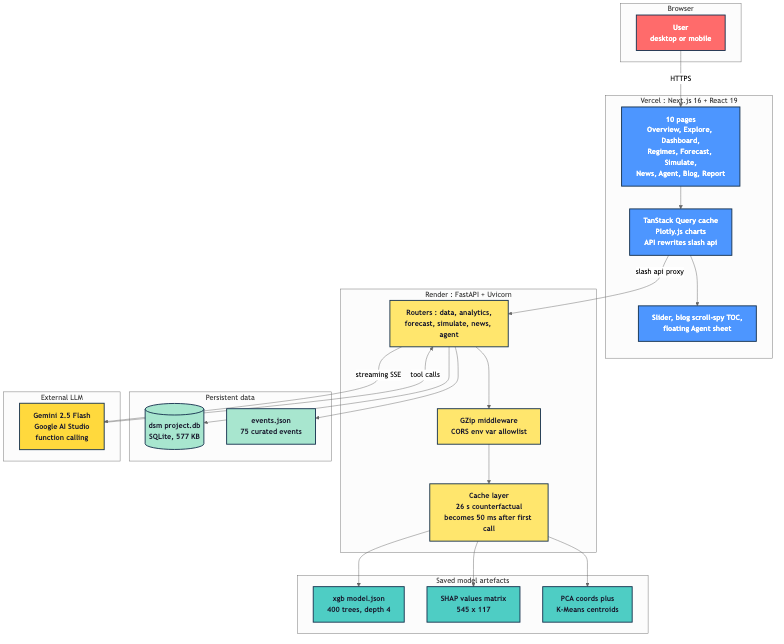
\includegraphics[width=\linewidth]{../diagram/system_architecture.png}
\caption{System architecture. The browser talks to a Next.js
front-end on Vercel, which proxies API calls to a FastAPI backend on
Render, which in turn queries SQLite, the saved XGBoost and SHAP
artefacts, and Gemini 2.5 Flash for the agent path.}
\label{fig:system-architecture}
\end{figure}

The system is a clean two-tier split. The presentation tier is a
Next.js 16 application with React 19, Tailwind CSS, Plotly.js for
interactive charts, and TanStack Query for data fetching and caching.
The data and inference tier is a FastAPI application running under
Uvicorn, which exposes six routers (data, analytics, forecast,
simulate, news, agent), a Gemini 2.5 Flash function-calling agent, and
the saved model artefacts (XGBoost JSON, SHAP value matrix, K-Means
centroids, walk-forward predictions). All persistence sits in a
single committed SQLite file plus a small \texttt{saved\_model}
folder.

\subsection{Data lineage from pipeline to dashboard}

\begin{figure}[H]
\centering
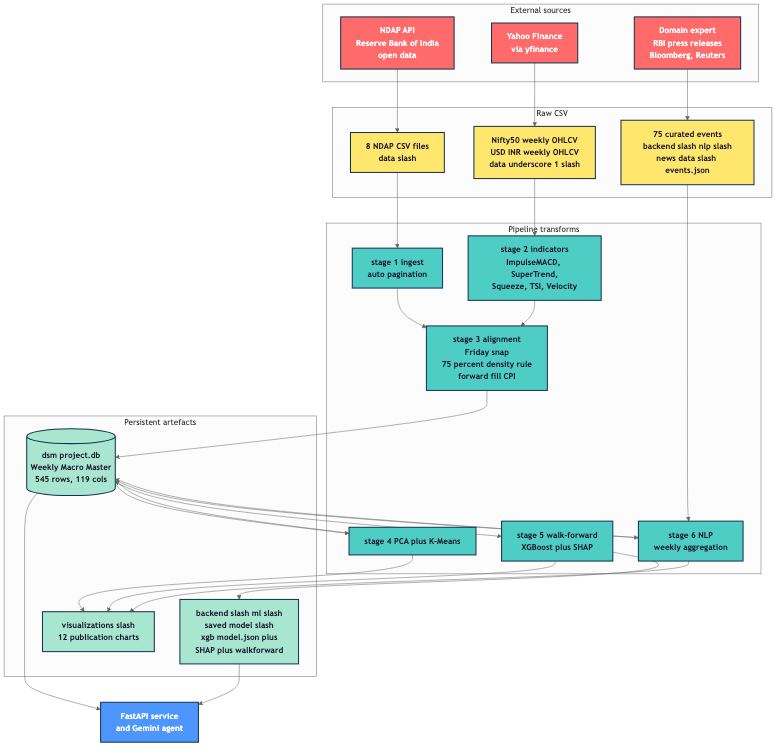
\includegraphics[width=\linewidth]{../diagram/data_lineage.png}
\caption{End-to-end lineage. Raw CSVs flow through six pipeline
stages into SQLite and the saved-model folder; the FastAPI service
reads from both and exposes the data through typed routes.}
\label{fig:data-lineage}
\end{figure}

The lineage is intentionally one-directional. No live request mutates
the database. A new analysis run rebuilds the SQLite table from
scratch from the CSV cache, which keeps the deployed application
deterministic.

\subsection{Frontend pages}

The dashboard exposes ten pages, each scoped to a single analytical
question.

\begin{table}[H]
\caption{Frontend pages with one-line descriptions and the public URL
suffix on \texttt{dsm-project-phi.vercel.app}.}
\label{tab:frontend-pages}
\renewcommand{\arraystretch}{1.18}
\rowcolors{2}{SoftGray}{white}
\begin{tabularx}{\linewidth}{@{} l l Y @{}}
\toprule
\rowcolor{Slate}\color{white}\textbf{Page} &
\color{white}\textbf{Path} &
\color{white}\textbf{Purpose} \\
\midrule
Overview & \texttt{/} & Editorial landing page with live hero chart and project summary. \\
Data Explorer & \texttt{/explore} & Sortable, filterable table of the 545 by 119 panel, exportable to CSV. \\
Dashboard & \texttt{/dashboard} & Interactive time-series, correlation heatmap, and distribution explorer. \\
Regimes & \texttt{/regimes} & Live PCA scatter plus regime fact-sheets and per-regime statistics. \\
Forecast \& SHAP & \texttt{/forecast} & Walk-forward actual versus predicted, interactive SHAP bar chart, single-row waterfall. \\
Simulate & \texttt{/simulate} & The headline feature, a policy counterfactual slider with response curve, confidence interval, and SHAP attribution. \\
News \& NLP & \texttt{/news} & Seventy-five curated events, sentiment timeline, and category filter. \\
Agent & \texttt{/agent} & Gemini 2.5 Flash chat with function-calling against the dataset. \\
Blog & \texttt{/blog/wacmr-investigation} & Long-form technical write-up with embedded charts and a sticky scroll-spy table of contents. \\
Report & \texttt{/report} & The full generated research report, rendered with all twelve figures and two summary tables. \\
\bottomrule
\end{tabularx}
\end{table}

\subsection{The counterfactual simulator}

The \texttt{/simulate} page is the project's headline interactive
feature. The user moves a slider for the policy Repo Rate change
(in basis points, from $-200$ to $+200$ in 25 bps steps) and the
system returns the model's counterfactual prediction for next week's
WACMR, a 90\% confidence interval, and a SHAP attribution showing
which features contribute to the change.

The implementation has one substantive engineering decision worth
documenting. A naive implementation that re-runs the full XGBoost
inference for every slider position takes about 26 seconds per call,
because the SHAP attribution involves iterating over every tree in
the model. A two-layer cache reduces this to roughly 50 milliseconds
in the steady state.

\begin{itemize}
\item \textbf{First layer, sweep precomputation.} The full slider
  sweep from $-200$ to $+200$ basis points is precomputed at
  deployment time and persisted as
  \texttt{simulate\_sweep\_default.json} in
  \texttt{backend/ml/saved\_model/}. Slider drags read directly from
  this JSON.
\item \textbf{Second layer, real-time debounce.} Slider updates are
  debounced at 120 milliseconds in the front-end so that rapid drags
  produce one final inference rather than a stream of intermediate
  ones. This keeps the 50 millisecond steady-state path responsive.
\end{itemize}

The 26-second to 50-millisecond improvement is roughly $500\times$
and is what makes the slider feel like a real interactive widget.

\subsection{The Gemini-powered data agent}

The \texttt{/agent} page wraps Gemini 2.5 Flash in a function-calling
loop with seven typed tools. The agent can answer free-form questions
about the dataset, run arbitrary read-only SQL, fetch SHAP
contributions for any row, run a counterfactual at any policy delta,
look up regime statistics, and search column names by fuzzy match.

\begin{figure}[H]
\centering
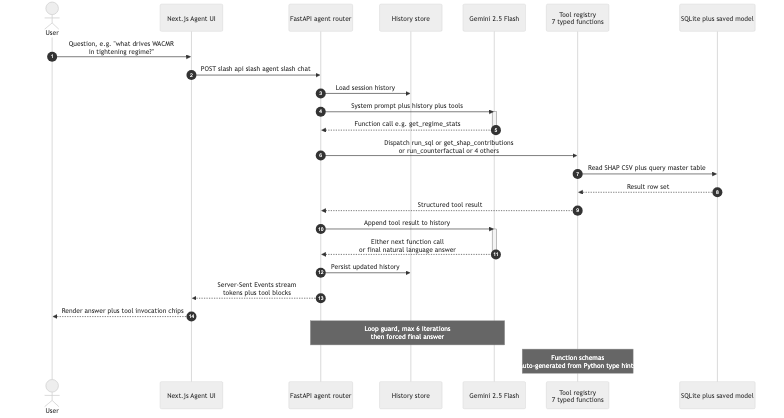
\includegraphics[width=\linewidth]{../diagram/agent_loop.png}
\caption{Gemini function-calling loop. The user's question enters the
loop on the left; tool calls and final answer stream back as
Server-Sent Events. A loop guard caps iterations at six to bound
worst-case latency.}
\label{fig:agent-loop}
\end{figure}

The seven tools are listed below, with the underlying implementation
file in \texttt{backend/agent/tools.py}. Function schemas are
auto-generated from Python type hints, so adding a new tool is a
matter of writing one Python function with annotated parameters.

\begin{itemize}
\item \texttt{run\_sql(query: str) -> rows}: read-only SQL against
  the master table; the tool refuses INSERT, UPDATE, DELETE, and DDL.
\item \texttt{run\_counterfactual(repo\_rate\_delta\_bps: float) -> dict}:
  invokes the cached counterfactual simulator and returns the
  prediction with a 90\% CI.
\item \texttt{get\_shap\_contributions(week\_date: str) -> list}: SHAP
  decomposition for the specified row.
\item \texttt{compare\_regimes(column: str) -> dict}: per-regime
  descriptive statistics for any chosen column.
\item \texttt{semantic\_column\_search(term: str) -> list}: fuzzy-match
  against the column registry; supports synonyms (``inflation'' maps
  to CPI columns).
\item \texttt{describe\_schema(category: str) -> list}: returns column
  metadata, optionally filtered by category.
\item \texttt{plot\_chart(...) -> dict}: renders an interactive Plotly
  chart directly in the chat interface.
\end{itemize}

The system prompt in \texttt{backend/agent/system\_prompt.md} casts
the agent as a research analyst rather than a generic chatbot, with
explicit instructions to ground every numeric claim in either a tool
call or a verbatim quote from the dataset, and to refuse questions
that fall outside the WACMR domain.

\subsection{Blog and live report}

Beyond the dashboard, two long-form pages document the investigation
itself. The \texttt{/blog/wacmr-investigation} page is an eleven-section
technical narrative with embedded live plots, a sticky scroll-spy
table of contents that highlights the user's current section, and an
embedded counterfactual widget that lets the reader play with the
model inline. The \texttt{/report} page renders the complete generated
research report with all twelve pipeline figures and the two summary
tables (datasets and performance), again with a sticky table of
contents and full hyperlinks.

\begin{finding}
The deliberate choice to publish both a blog (which favours narrative
and inline interactivity) and a report (which favours structure and
references) reflects the two distinct audiences for the work. The
blog is for non-specialists who want to understand what was done; the
report is for evaluators and researchers who want the full provenance
and the reproducibility trail.
\end{finding}
